% mainfile: ../ltexpprt.tex

One of the key challenges while creating a prospective ILI case count
predictor is the fact that the official estimates are often 
delayed and furthermore even when published the estimates are revised
over a number of weeks before these are finally stabilized.
For this paper, we concentrate on 15 Latin American countries 
as described in Section~\ref{sec:experiments} and consider the official 
ILI estimates from the Pan American Health Organiation (PAHO)~\cite{PAHO:2013}.
%One of the problems with PAHO count dataset is that PAHO count value of a
%specific week may change over time. In other words, PAHO count values are
%unstable for a period of time after they are published for the first time.
Thus we can categorize PAHO count values downloaded on any week
into three different types: (a) the uknnown
PAHO counts reprenseted  by $\ddot{P}_t$, (b) the known and stable PAHO counts
denoted by $\dot{P}_t$, and (c) the known and unstable PAHO counts denoted by
$\tilde{P}_t$. While we want to predict $\ddot{P}_t$, the uncertainity associated
with $\tilde{P}_t$ introduces errors in the predictions. In this section, 
we study the effects of these ``unstable'' data and propose 
three different models to adjust these unstable
values to more accurate ones.

%In order to study the stability behavior of PAHO data, we start with plotting
%relative error of PAHO count values with respect to the stable values. Relative
%error is defined as follows:

%\begin{equation}
%E_{relative} = \frac{\tilde{P}_i - \dot{P}_i}{\dot{P}_i}
%\end{equation}
Figure~\ref{fig:relerrors}, plots the relative error of the unstable Paho data over
its final estimate as a function of time. While it can be seen that different countries 
have different stability characteristics: 
for some countries, PAHO count values are
stabilized very slowly while for others, they are stabilizing faster, as the number of 
updates for a particular week increases, the values generally stabilize.
Stability behavior of PAHO count values were also found to be dependent on the 
time of the year as shown in Figure~\ref{fig:seasonal_relerrors}.
To plot this curve for Argentina, we categorized any week with less than 100 cases to be a low season,
greater than 300 tobe a high season and the remaining values to be low season (the thresholds
were different for different countries).

% talking about priliminary results
\begin{figure}[h]
  \centering
   \begin{tabular}{cc}
     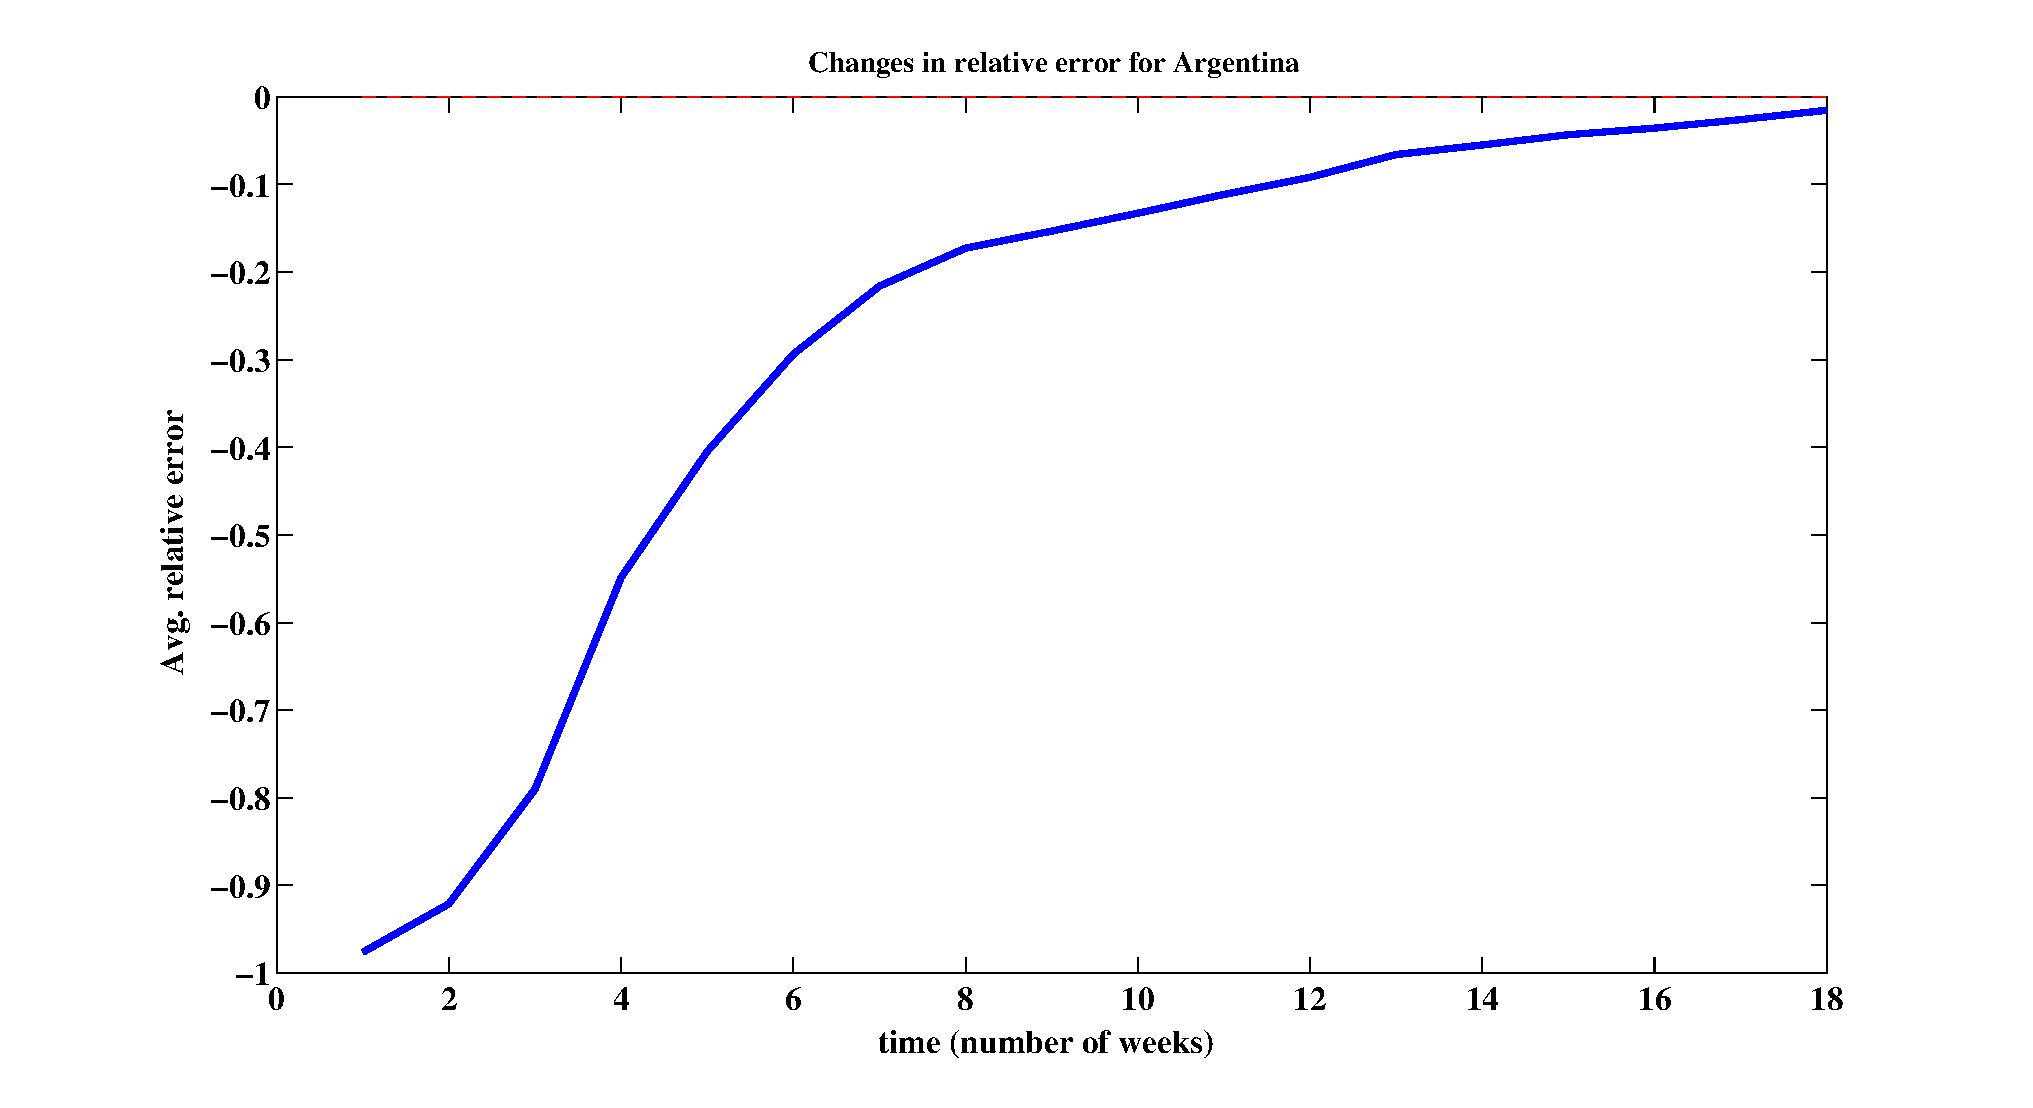
\includegraphics[width=.45\columnwidth]{fig/forpaper_AVGrelativeALLs_Argentina.eps} &
     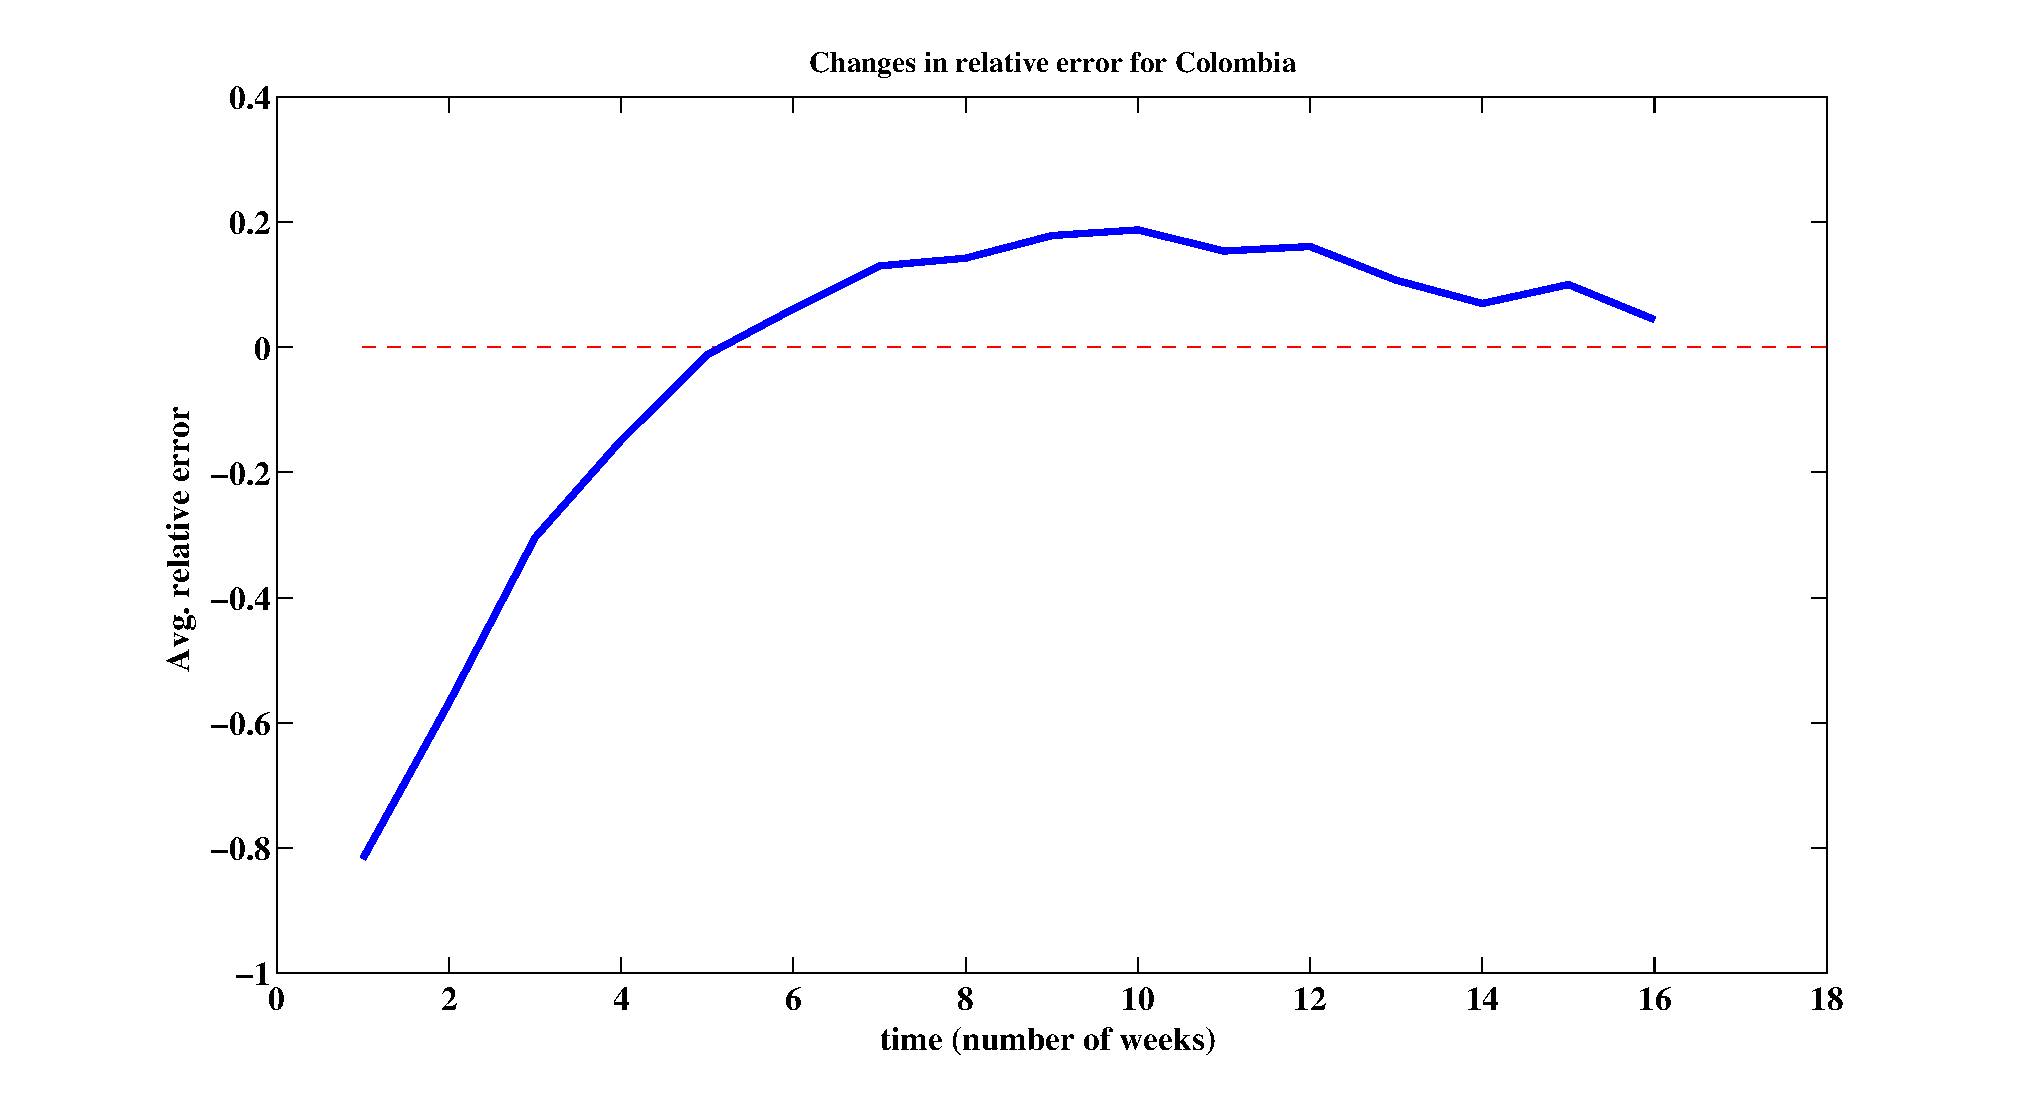
\includegraphics[width=.45\columnwidth]{fig/forpaper_AVGrelativeALLs_Colombia.eps} \\
 %    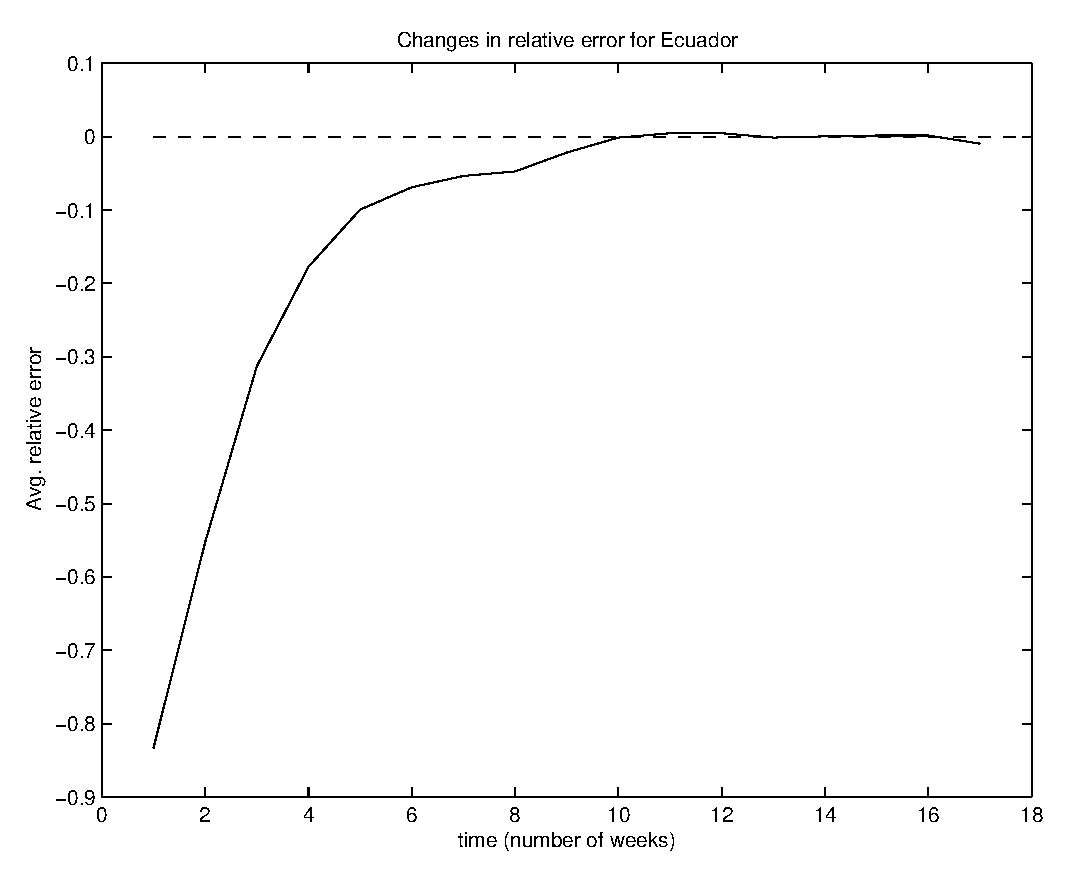
\includegraphics[width=.23\textwidth]{forpaper_AVGrelativeALLs_Ecuador.eps} &
 %    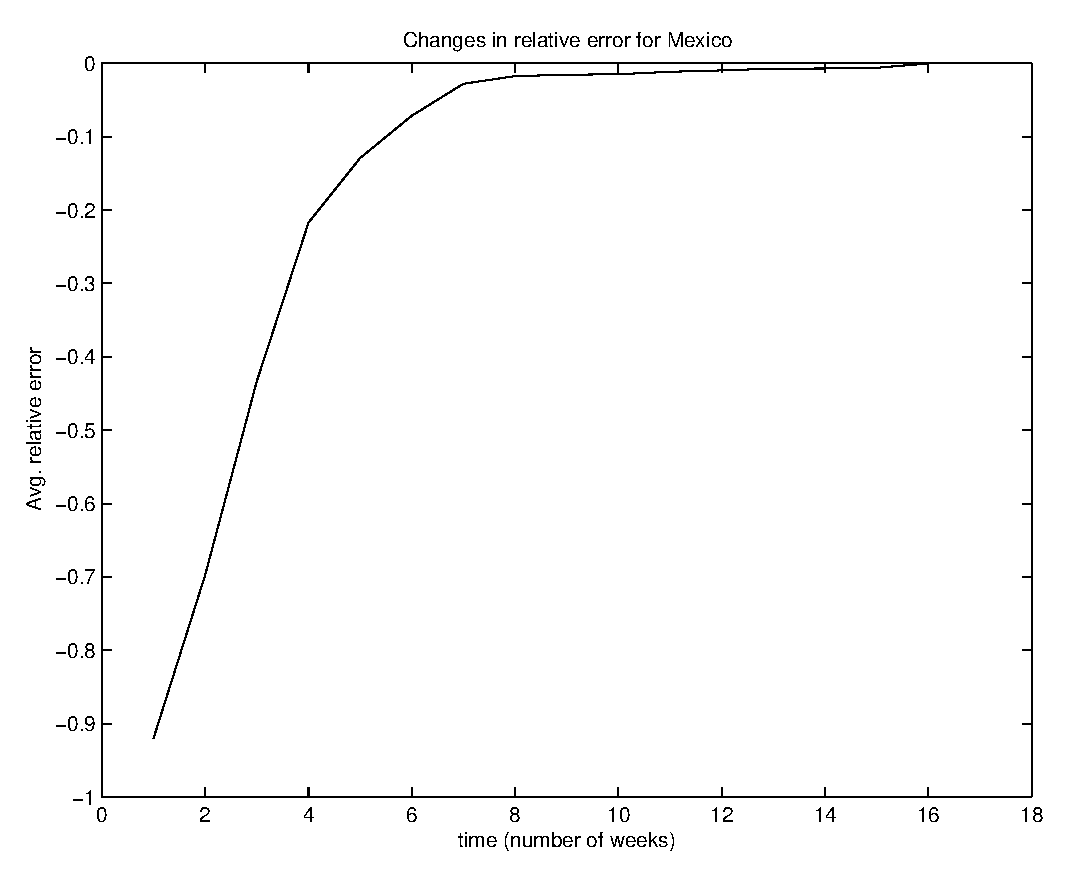
\includegraphics[width=.23\textwidth]{forpaper_AVGrelativeALLs_Mexico.eps} \\
      (a) & (b) \\ %& (c) & (d) \\
  \end{tabular}
  \caption{Average relative error of PAHO count values with respect to stable values.
  (a) Argentina,
  (b) and Colombia.
%  (c) Ecuador, and
%  (d) Mexico.
  \label{fig:relerrors}
  }
\end{figure}

\begin{figure}[h]
  \centering
    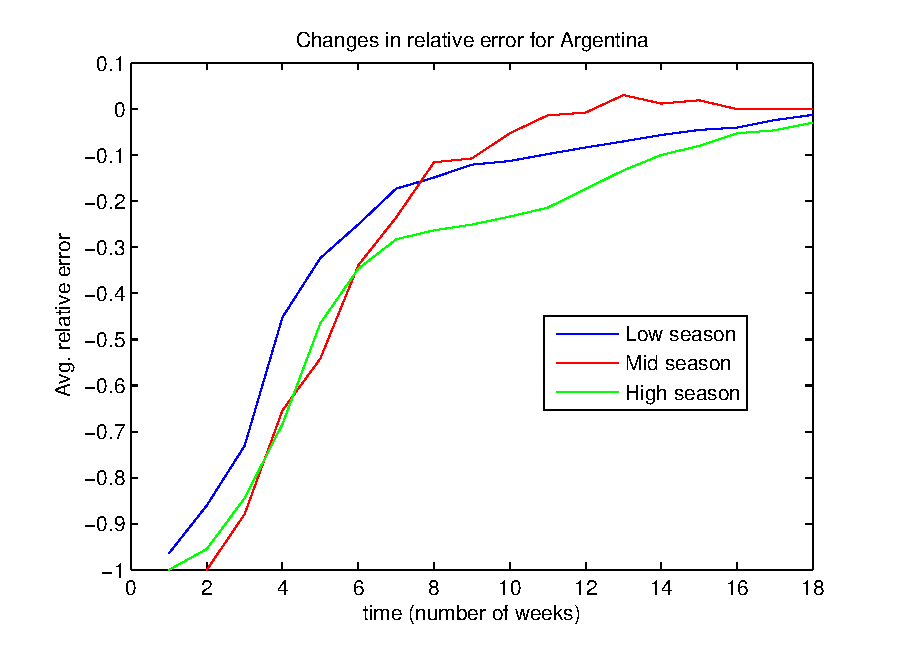
\includegraphics[width=0.5\textwidth]{fig/forpaper_seasonalAVGrelativeALLs_Argentina.eps}
  \caption{Average relative error of PAHO count values for Argentina with respect
  to their stable values for low, mid, and high seasons.}
  \label{fig:seasonal_relerrors}
\end{figure}  

% waiting for publishing stable PAHO values does not work because it is too late

At the same time, the official estimates provide an estimate of number of samples
used to generate the estimate. Preliminary experiments show that
this size is correlated with the accuracy of ILI case counts. In other words,
in general, larger values of statistical population size results in smaller
relative errors for ILI case count.Thus using both the number of samples and the lag in 
uploading the week data, we can use machine learning techniques to revise the officially 
published PAHO estimates. Preliminary results
show that for different seasons and different countries, we have different
stability patterns. Therefore, any PAHO count adjustment method should be
customized for seasons and countries separately. 

Let us assume that $\dot{\mathcal{P}}$ is the set of stable PAHO counts for a
specific country. Also, assume that sequence of updates for each stable PAHO
count value is available. In other words, for $\dot{P}_i$ we have the following
set:
 
\begin{equation}
\dot{\mathcal{P}}_i = \left \{P_i^{(1)},P_i^{(2)},...,P_i^{(m)},...  \right \}
\end{equation}

where, $P_i^{(m)}$ is the value of $P_i$ after $m$ weeks of update. 
For each stable PAHO count value, $\dot{P}_i$, there is a threshold, 
$\dot{T}_i$ that for $m \ge \dot{T}_i$, $P_i^{(m)}$ is stable.

Hence, we have:
\begin{equation}
\dot{\mathcal{P}}_i = \left \{P_i^{(1)},P_i^{(2)},...,P_i
^{(\dot{T}_i-1)},\dot{P}_i,\dot{P}_i,...  \right \}
\end{equation}

In other words, $P_i$ is stabilized after $\dot{T}_i$ weeks.



After recognizing high, low, and mid-season months for the country, we can
categorize each $\dot{P}_i$ to belong to one of these categories. Then, for
category S, an adjustment dataset is constructed named as $\mathcal{P}_A{^S}$
which is defined as follows:

\begin{equation}
\mathcal{P}_A{^S} = \left \{ (1,P_i^{(1)},\dot{P}_i,N_i^{(1)}),...,(m,P_i^{(m)},\dot{P}_i,N_i^{(m)}), ...  \right \}
\end{equation}

Each member of $\mathcal{P}_A{^S}$ is a tuple with four items: first item shows
the time slot that the sample belongs to, second item is the actual unstable
value of $P_i$, third item is the related stable value, and last item,
$N_i^{(m)}$, is the size of statistical population at that week.

In the next step, a linear regression algorithm is used to adjust unstable PAHO
values. In order to adjust value of the PAHO values in the $m$th time slot of
season S, we use $\mathcal{P}_A{^S}$ set to learn $a_0$, $a_1$, $a_2$, and
$a_3$ coefficients in the following equation:

\begin{equation}
\hat{\dot{P}}_i^{(m)} = a_0 + a_1 \times m + a_2 \times P_i^{(m)} + a_3 \times N_i^{(m)}
\label{eq:correctionpaho}
\end{equation}

where, $\hat{\dot{P}}_i^{(m)}$ is the adjusted PAHO count value for the $m$th time slot.

Experimental results show that this adjustment method results in more accurate
known PAHO values. Average relative errors of the published unstable PAHO
values before and after correction for each
country is shown in Figure ~\ref{fig:avgrelerrors}.

%Some experimental results are shown in Figure ~\ref{fig:adjustedrelerrors}.

\begin{figure}[h]
  \centering
    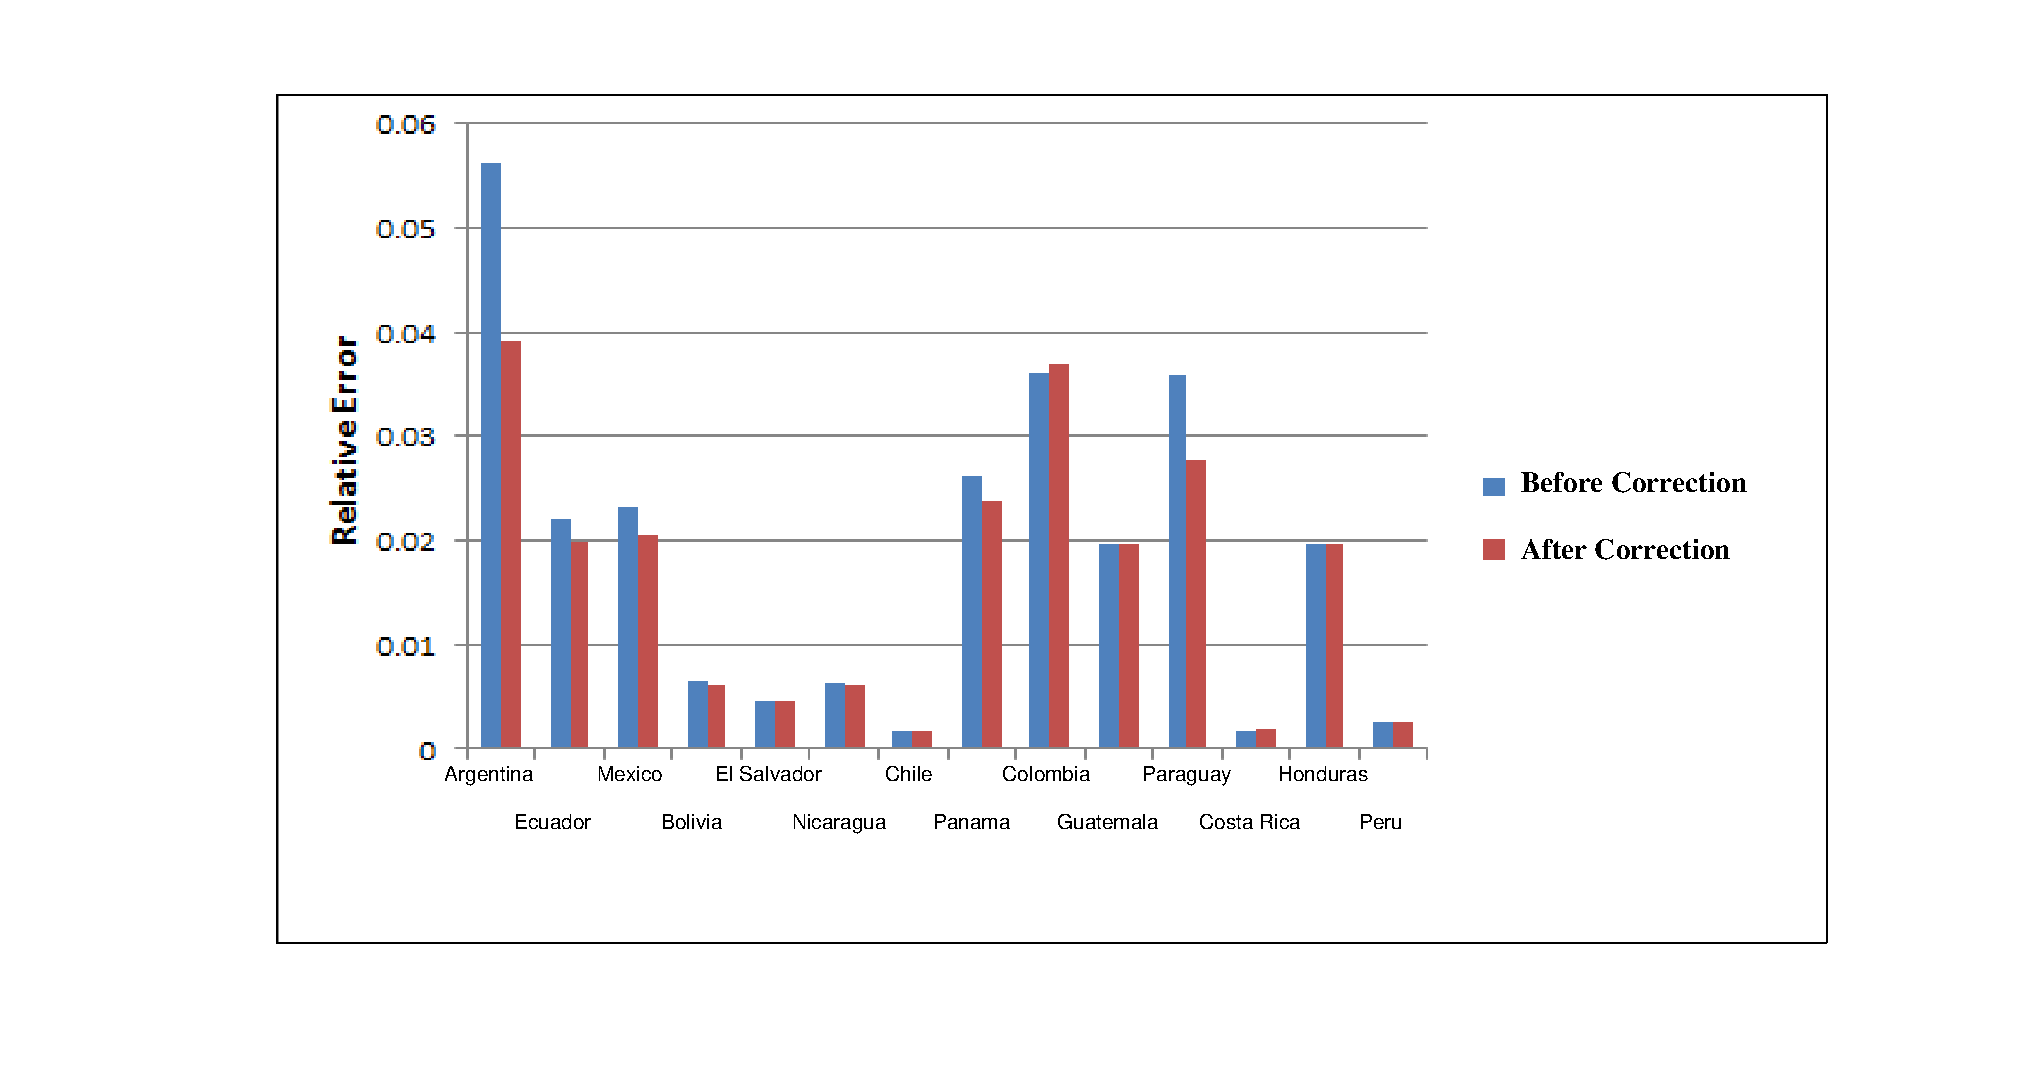
\includegraphics[width=0.5\textwidth]{fig/errs.eps}
  \caption{Average relative error of PAHO count values before and after 
  correction for different countries.}
  \label{fig:avgrelerrors}
\end{figure}

Similar to Eq.~\ref{eq:correctionpaho}, in addition to $P_i^{(m)}$, one can
use only time difference ($m$) or size of population ($N_i^{(m)}$) to correct
unstable PAHO values. Effect of these corrections on overall accuracy of
predictions are shown in Section ~\ref{sec:results}.
